\documentclass{article}

\usepackage{amssymb} %chekmark symbol
\usepackage{graphicx}

\begin{document}

\date{versie 8 april 2015}
\title{low-level scenario FR-U007}
\maketitle


%%%%%%%%%%%% AUTHOR GRAPH
\subsubsection*{AUTHOR GRAPH}
\vspace{2 mm}

\textbf{ID}: FR-U007
\vspace{2 mm}

De author graph van een gebruiker visualiseert het netwerk van de gebruiker in een graaf waarvan de nodes (co-)auteurs zijn en de edges de publicaties die ze samen publiceerden. 


\begin{figure}[!h]
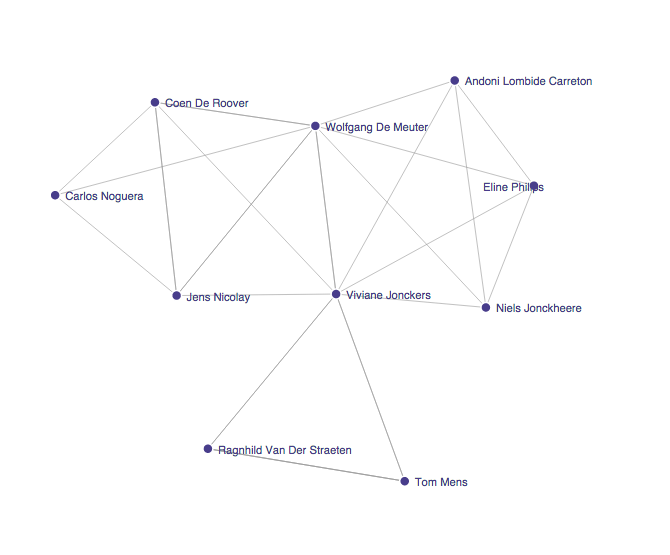
\includegraphics[width=1.1\textwidth]{basicGraph.png}
\end{figure}



\hrule
\vspace{2 mm}
\noindent \textbf{Scenario}:
\begin{description}
\item CLIENT : G wil graph weergeven (open 'graph view')
	\begin{description}
	\item $\rightarrow$ graph data moet opgehaald worden van server
	\item ! D3 moet geladen worden -> check compatibiliteit 
	\end{description}
	
\item SERVER : 
	\begin{description}
	\item $\leftarrow$ json met graph data 
		\begin{description}
		\item [$\cdot$] de data voor de graaf bestaat uit, vertrekkende van de gebruiker, alle auteurs waarmee deze verbonden is via co-auteurschap en bijhorende publicaties, en dit transitief tot op een bepaalde diepte. 
		\item [$\cdot$] het algoritme van de D3.js library visualiseert een \emph{gerichte} graaf, terwijl de co-auteur relatie ongericht is. Om dit op te lossen moet het JSON bestand data voor een graaf bevatten waarvan slechts 1 van beide richtingen gespecificeerd is (i.e. link van de ene co-auteur naar de andere, maar niet andersom). Dit wordt dan gevisualiseerd met een lijn zonder pijltje, dus alsof het een link is die voor beide richtingen geldt.  
		\item [$\cdot$] een voorbeeld en test JSON is te vinden op github 
		\item [$\cdot$] hier moet misschien nog een author ID aan toegevoegd worden (?)
		\end{description}
	\end{description}
	 
\item CLIENT : 
	\begin{description}
	\item visualisatie van de graph
	\item gebruiker klikt op
		\begin{description}
		\item  [$\cdot$] een node die overeen stemt met een auteur, maar niet met een gebruiker $\hookrightarrow$ A1
		\item  [$\cdot$] een node die overeen stemt met een gebruiker $\hookrightarrow$ A2
		\item  [$\cdot$]een edge tussen twee auteurs die (een lijst van) publicatie(s) voorstelt $\hookrightarrow$ B
		\end{description}
	\end{description}
	
\hrule
\vspace{2 mm}
 
\item A1: click op auteur, maar geen gebruiker
\item  CLIENT : 
	\begin{description}
	\item $\rightarrow$ get info van auteur via authorID (lijst van publicaties?)
	\end{description}
	
\item SERVER : 
\begin{description}
	\item $\leftarrow$ info auteur
	\end{description}
	
\item CLIENT :  
	\begin{description}
	\item display auteursinfo
	\end{description}
	
\hrule
\vspace{2 mm}


\item A2: click op auteur, gebruiker
\item  CLIENT : 
	\begin{description}
	\item $\rightarrow$ get info van auteur via authorID (lijst van publicaties?)
	\end{description}
	
\item SERVER : 
\begin{description}
	\item $\leftarrow$ info auteur en accountinfo gebruiker 
	\end{description}
	
\item CLIENT :  
	\begin{description}
	\item display auteursinfo + COMPACT PROFILE VIEW (affiliatie, deel portfolio e.d.)
	\end{description}
	
\hrule
\vspace{2 mm}


\item B: click op link die publicaties voorstelt
\item  CLIENT : 
	\begin{description}
	\item $\rightarrow$ get (array van) publicatie metadata adhv pubId
	\end{description}
	
\item SERVER : 
\begin{description}
	\item $\leftarrow$ array van publicatie metadata 
	\end{description}
	
\item CLIENT :  
	\begin{description}
	\item metadata preview (mogelijks van meerdere publicaties?)
	\end{description}
	
\end{description}

\end{document}

